\chapter{Анализ безопасности WEP}

Атаки на протокол WEP можно классифицировать следующим образом
(рисунок~\ref{fig:wep_attacks_classification}):

\begin{itemize}
    \item с восстановлением ключа и без восстановления ключа;
    \item активные и пассивные;
    \item на точку доступа и на клиентов точки доступа.
\end{itemize}

Активные --- это атаки, позволяющие получить данные, передаваемые в сети, или
отправлять легальные пакеты в сеть без знания ключа шифрования.  Пассивные ---
позволяют получить ключ подключения к сети. Атаки без восстановления ключа
позволяют значительно ускорить процесс накопления векторов инициализации для
пассивных атак.

\begin{figure}
    \includegraphics[width=1\textwidth]{graphics/wep_attacks_classification.eps}
    \caption{Классификация атак на протокол WEP}
    \label{fig:wep_attacks_classification}
\end{figure}

Большинство современных реализаций стека TCP/IP генерируют некоторый объем
сетевого трафика при подключении к сети. Примером могут служить сообщения
протоколов DHCP, NetBIOS, IPv6 NDP и так далее. Однако количество передаваемых в
этом случае пакетов (как правило, до нескольких десятков) недостаточно для
проведения KoreK-атаки, требующей десятки тысяч пакетов с различными векторами
инициализации.

Стандартный подход, заключающийся в передаче перехваченных ранее
широковещательных пакетов, в рассматриваемом случае также бесполезен. Поскольку
точка доступа контролируется злоумышленником, все ретранслированные ею пакеты
будут использовать ключ WEP, не представляющий интереса для злоумышленника.
Таким образом, для взлома WEP необходимо спровоцировать подключившегося клиента
на передачу достаточного количества пакетов с различными значениями векторов
инициализации. Решить эту задачу можно путём передачи клиенту сообщений,
требующих ответа (ARP, ICMP-Echo, IPv6 NDP). Но сделать это необходимо без
знания ключа WEP.


\section{Атаки без восстановления ключа}

\subsection{Атака с фрагментацией}

Существует достаточно много методов формирования пакетов WEP без знания ключа
шифрования. Наиболее эффективным является использование фрагментации на
канальном уровне 802.11 [2][4]. Суть этого метода заключается в эксплуатации атаки с
известным открытым текстом. Используя предсказуемый формат заголовков LLC,
существует возможность восстановить 8 байт гаммы (выхода алгоритма PRGA в RC4,
далее PRGA), рисунок~\ref{fig:restore_part_of_gamma}. Для этого первые восемь из
зашифрованных байт складываются по модулю два с константой, содержащей
стандартное значение заголовков LLC.

%{Перехват необходимых пакетов}

Как видно из рисунка~\ref{fig:default_llc_header}, в заголовке LLC два последних байта могут меняться. Их
значение определяет тип используемого протокола вышестоящего уровня. Возможные
значения данных полей описаны в документах IANA.

\begin{figure}
    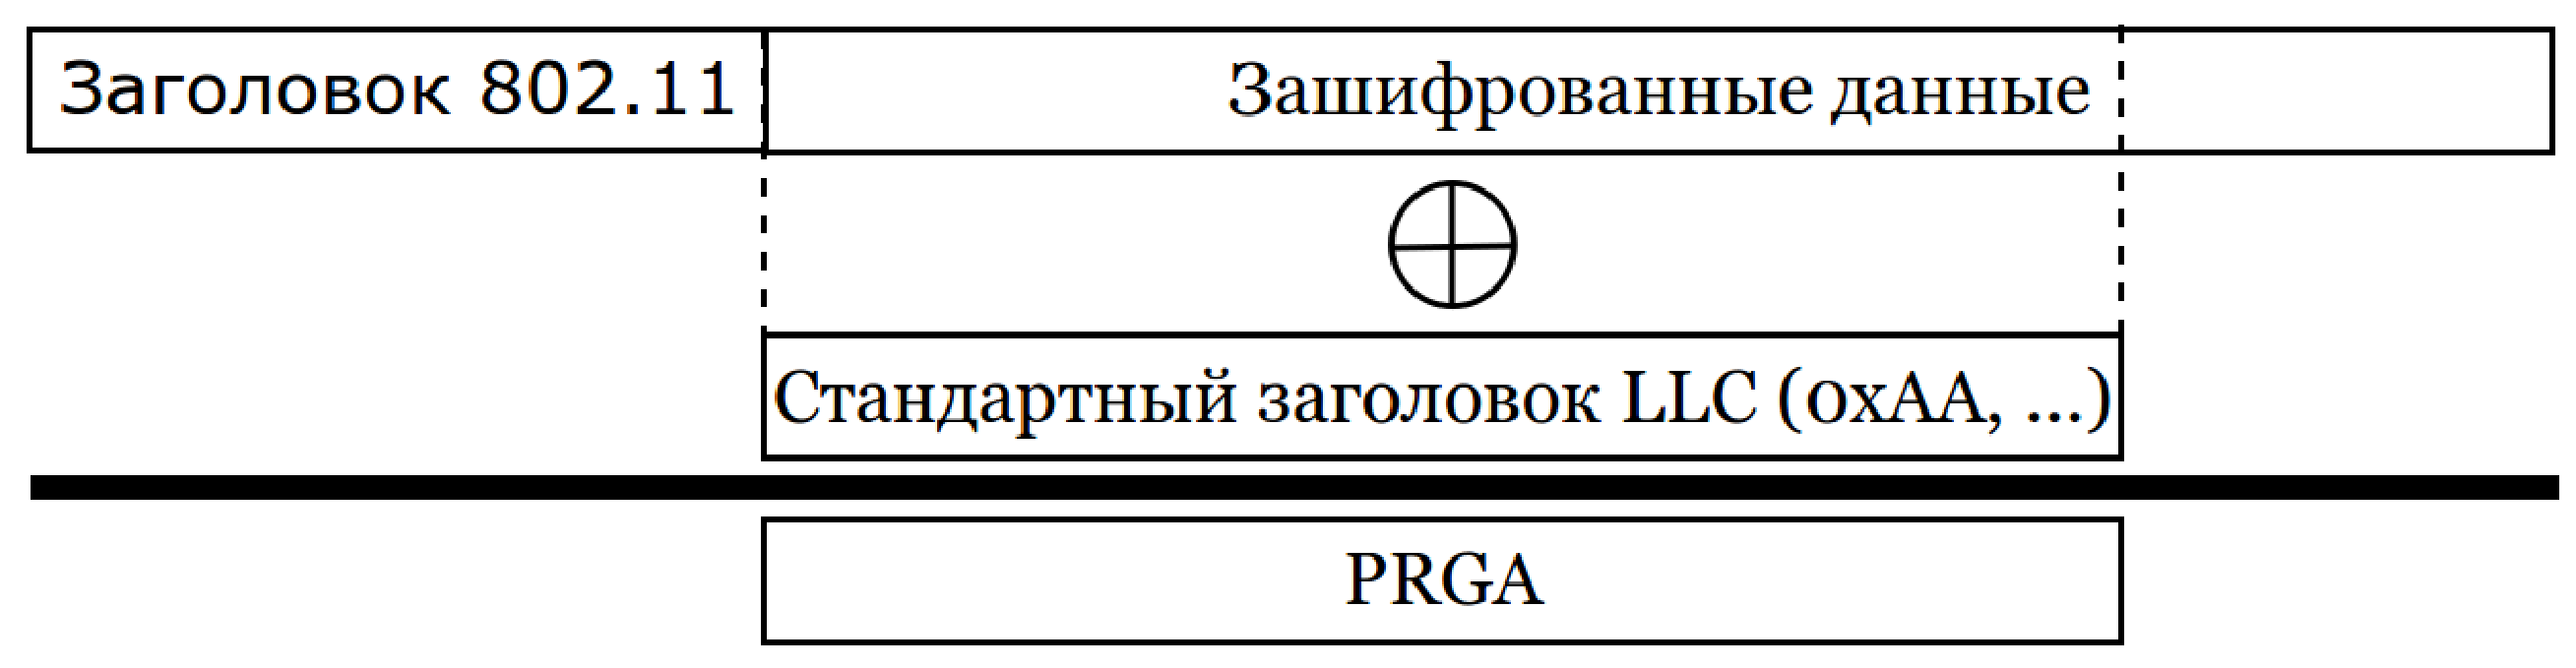
\includegraphics[width=1\textwidth]{graphics/restore_part_of_gamma.eps}
    \caption{Восстановление отрезка гаммы}
    \label{fig:restore_part_of_gamma}
\end{figure}

\begin{figure}
    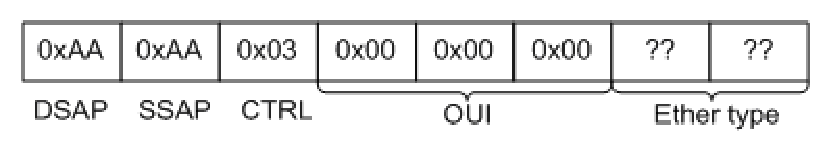
\includegraphics[width=1\textwidth]{graphics/default_llc_header.eps}
    \caption{Стандартный заголовок LLC (802.2 snap)}
    \label{fig:default_llc_header}
\end{figure}

В большинстве случаев беспроводные сети используются для передачи IP-трафика.
Следовательно, поле Ether type может принимать одно из трёх возможных значений:

\begin{itemize}
    \item 0x0800 --- при передаче IP-пакетов;
    \item 0x0806 --- для пакетов ARP;
    \item 0x86DD --- для пакетов IPv6.
\end{itemize}

Пакеты ARP легко отличить от других по их фиксированной длинне (28 байт
данных). Использование протокола IPv6 достаточно просто идентифицируется по
наличию широковещательных пакетов на MAC-адреса 33:33:xx:xx:xx:xx, используемых
протоколом IPv6 NDP. Полученные 8 байт гаммы могут быть использованы для
передачи в сеть произвольных данных той же длины. Но с практической точки зрения
это не представляет большого интереса, поскольку все 8 байт в передаваемом
пакете будет занимать заголовок LLC. Чтобы обойти это ограничение, может
использоваться функция фрагментации на канальном уровне. Беспроводные сети
реализуют механизм, позволяющий передать один пакет вышестоящего уровня в
нескольких (до 16) фрагментах 802.11. После перехвата одного из пакетов клиента
и восстановления PRGA, отправляемый пакет разделяется на несколько фрагментов,
содержащих по 4 байта данных (рисунок~\ref{fig:send_fragmented_frames}).

\begin{figure}
    \includegraphics[width=1\textwidth]{graphics/send_fragmented_frames.eps}
    \caption{Передача фрагментированных фреймов}
    \label{fig:send_fragmented_frames}
\end{figure}

Каждый их них передается как отдельный фрейм с использованием функции
фрагментации 802.11. Пакеты дополняются контрольной суммой (WEP ICV) и
зашифровываются с использованием отрезка восстановленной гаммы. Таким образом,
без знания ключа WEP в сеть можно передать пакеты длиной до 64 байт. На практике
в сеть можно передать пакеты большего размера. Для этого используется
IP-фрагментация, а также структура некоторых служебных пакетов. Например, при
перехвате пакета ARP пакета можно восстановить не 8, а 24 байта гаммы
(рисунок~\ref{fig:arp_packet}). Для этого используются крайне предсказуемые
значения заголовков LLC, ARP, а также MAC-адрес отправителя, указанный в
заголовках 802.11 в открытом виде.

\begin{figure}
    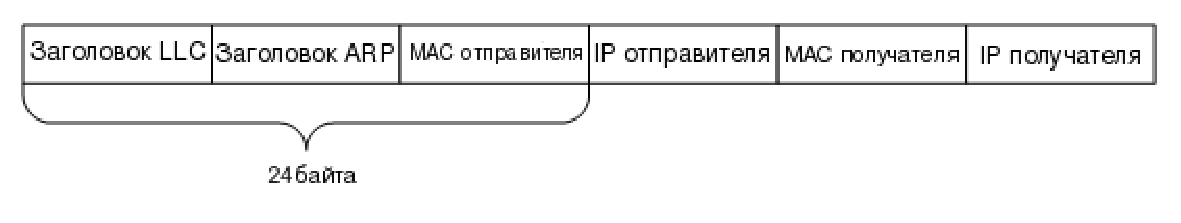
\includegraphics[width=1\textwidth]{graphics/arp_packet.eps}
    \caption{Пакет ARP}
    \label{fig:arp_packet}
\end{figure}

При использовании в сети IPv6 можно восстановить и больший отрезок гаммы.
Например, при перехвате пакетов IPv6 NDP Neighbor Solicitation или Router
Solicitation можно восстановить до 50 байт гаммы (заголовки LLC + заголовки IP +
2 байта заголовков ICMP). Это связанно с тем, что в заголовке IPv6 отсутствует
поле контроля целостности. Кроме того, при использовании Local-Link адресации
адрес IPv6 можно восстановить по MAC-адресу в заголовках 802.11, если узлом не
используется механизмы рандомизации адресов. Отличить разные типы сообщений IPv6
можно по MAC-адресам получателей и размеру. Например, пакет, IPv6 Router
Solicitation имеет длину 70 байт и передается на MAC-адрес 33:33:00:00:00:02.

С использованием 50 байт PRGA в сеть можно передать пакеты размером до 736 байт
((50-4)*16), что более чем достаточно для практических целей.

%{Генерация трафика}

При использовании атаки с фрагментацией у злоумышленника, установившего ложную
точку доступа, появляется возможность передать подключившейся станции
зашифрованный пакет, которой будет гарантированно обработан получателем. Таким
образом, остается только сформировать пакет, на который клиент ответит. Примером
подобного пакета является ARP-запрос. Дополнительным плюсом является тот факт,
что ARP-пакеты не блокируются персональными межсетевыми экранами. Однако для
того, чтобы станция ответила на ARP-запрос, необходимо, чтобы поле Target IP
содержало текущий IP-адрес интерфейса. Этой информацией злоумышленник не
обладает, поскольку адрес передается в пакетах в зашифрованном виде.

Чтобы получить IP-адрес станции, можно воспользоваться ARP сканированием, то
есть отправкой ARP-запросов на различные адреса получателей, и ожиданием ответа
на один из них. Если ответ был получен, значит, станция использует запрошенный
IP-адрес (например, 169.254.5.9, см. рисунок~\ref{fig:arp_scanning}).

\begin{figure}
    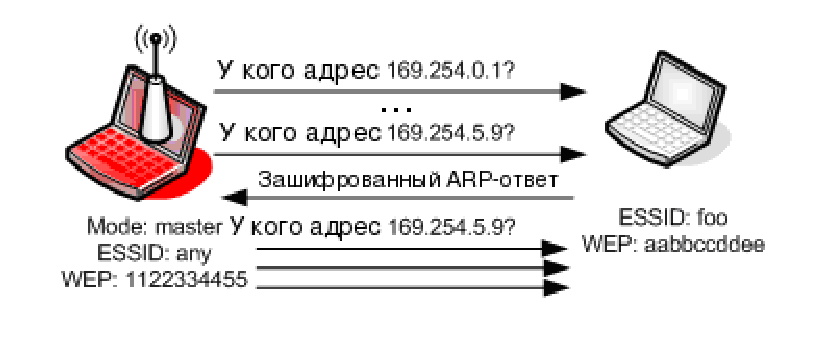
\includegraphics[width=1\textwidth]{graphics/arp_scanning.eps}
    \caption{ARP-сканирование}
    \label{fig:arp_scanning}
\end{figure}

В качестве диапазонов для сканирования могут выбираться адреса из диапазона
APIPA (169.254.0.0/16) или распространённые адреса RFC 1918 (например,
192.168.0.0/16). После того, как IP-адрес станции был определён, используется
повторная передача ARP-запроса с целью получения необходимого для пассивных атак
количества пакетов с различными векторами инициализации. Для того, чтобы
отличить ARP-запросы, отправленные на разные IP-адреса, могут использоваться
различные MAC-адреса отправителя. В случае поддержки станцией IPv6 ситуация
упрощается. Поскольку большинство реализаций стека IPv6 отвечает на
широковещательные (например, направленные на адрес ff02::01, см.
рисунок~\ref{fig:ipv6_usage}) ICMPv6-echo запросы, то достаточно отправить
подобный пакет в сеть.

Также в IPv6 может применяться пакет IPv6 Neighbor Solicitation. В этом случае
подбирать IP-адрес нет необходимости, поскольку Local-Link IP-адрес может быть
определён по MAC-адресу станции.

\begin{figure}
    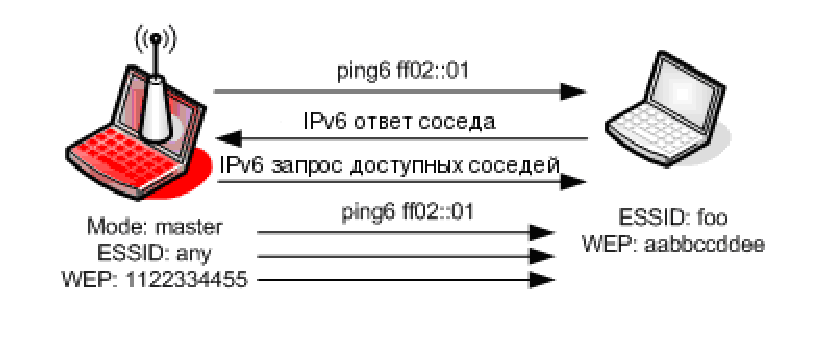
\includegraphics[width=1\textwidth]{graphics/ipv6_usage.eps}
    \caption{Использование IPv6}
    \label{fig:ipv6_usage}
\end{figure}

\subsection{Chopchop атака}

Chopchop атака, так же известна как chopping атака и атака KoreK, была
представлена в 2004 году человеком под псевдонимом KoreK. Данная атака позволяет
злоумышленнику интерактивно расшифровать последние $m$ байт зашифрованного
пакета, при этом потребуется отправить примерно $m*128$ пакетов в сеть. Атака не
получает ключ и не основана на специальных свойствах поточного шифра RC4.

Данная атака заключается в следующем: Перед шифрованием четырёхбайтовая
контрольная сумма CRC32, называемая ICV, добавляется в конец данных пакета. Пакет
с контрольной суммной P в конце может быть представлен как элемент
полиномиального кольца $F_2 |x|$. Если контрольная сумма верна, то $ P_{ONE} =
P\pmod{P_{CRC}}$, где $P_{ONE}$ является известным многочленом и $P_{CRC}$ тоже
известный неприводимый многочлен. Можно записать $P$ как $Q X^8 + R$, где $R$
--- последний байт $P$ и $Q$ --- все остальные байты. Когда зашифрованный пакет
  уменьшается на 1 байт с большой вероятностью контрольная сумма будет
  некорректной (см. рисунок~\ref{fig:wep_chopchop}).

\begin{figure}
    \includegraphics[width=1\textwidth]{graphics/wep_chopchop.eps}
    \caption{Chopchop атака: корректировка контрольной суммы CRC32}
    \label{fig:wep_chopchop}
\end{figure}

Допустим, что злоумышленник знает R, тогда если добавить $P_{ONE} +
(X^8)^{-1}(P_{ONE} + R)$ к $Q$, то контрольная сумма будет корректной. Данную
операцию можно выполнить на зашифрованном пакете. Если $R$ было выбрано
неправильно, то контрольная сумма будет некорректной.

Большиство точек доступа можно использовать для получения знания об отличии
между зашифрованным пакетом с корректной и некорректной контрольной суммой.
Например, если клиент не авторизован, и точка доступа получает пакет от этого
клиента, то точка доступа сгенерирует сообщение об ошибке. Пакеты с некорректной
контрольной суммой будут проигнорированы.

Злоумышленник может использовать эти знания для интерактивного расшифрования
пакетов. Злоумышленник выбирает полученный пакет для расшифрования, уменьшает
длинну пакета на 1 байт, угадывая $R$ и корректируя контрольную сумму пакета, и
отправляет пакет на точку доступа для проверки правильности угадывания $R$. Если
$R$ было угадано верно, то злоумышленник может расшифровать последний байт
данных и может продолжать с предпоследним байтом. Если $R$ было угадано неверно,
то берут сделующее значение $R$. После максимум 256 угадываний, а в среднем 128
угадываний, злоумышленник угадает значение $R$.


\section{Атаки с восстановлением ключа}

\subsection{FMS атака}

FMS атака, названная так от фамилий исследователей Fluhrer, Mantin и Shamir,
основана на уязвимости RC4 алгоритма. Исследователи обнаружили, что 9000 из
возможных 16 миллионов векторов инициализации можно считать слабыми и при
накоплении достаточного их количества позволяет вычислить ключ шифрования. Для
взлома ключа WEP в общем случае 5 миллионов зашифрованных пакетов должно быть
собрано для получения примерно 3000 слабых векторов инициализации (IV).

С определёнными векторами инициализации злоумышленник знает первый байт гаммы и
первые $m$ байт ключа позволяют получить $(m+1)$ый байт ключа за счёт уязвимости
в генераторе псевдослучайных чисел (PRNG) для генерации гаммы. Так как первый
байт открытого текста является частью WEP SNAP заголовка, злоумышленник может
предположить, что первый байт гаммы является $B \xor \text{0xAA}$. Таким образом,
злоумышленнику необходим вектор инициализации вида $(a+3, n-1, x)$, где индекс
ключа $a$ изначально равен $0$, $n=256$ и $x$ может принимать любое значение.
Получаем, что злоумышленнику необходимы векторы инициализации вида $(3, 255,
x)$. В WEP используются векторы инициализации длинной 24 бит (3 байта).

После третёх байт вектора инициализации, являющегося началом ключа, злоумышленник
может с некоторой вероятностью получить четвёртый байт ключа, используя гамму
$O$, вычисляя $K[i] = O-j-S[i]\pmod{n}$, где $i=3$ на этом шаге.

В данном случае злоумышленник не получает четвёртый байт ключа, так как этот
алгоритм не генерирует следующий байт ключа, а лишь угадывет возможное значение.
Можно повторить эти шаги с новыми пакетами и получить множество различных
возможных значений байта ключа. Наиболее часто встречающееся значение будет
правильным значением. После решения задачи получения четвёртого байта
злоумышленник аналогично решает задачу для получения пятого байта ключа.

Стоит заметить, что злоумышленник не может вычислять байты ключа в произвольном
порядке и ему нужны только сообщения со слабыми векторами инициализации. Таким
образом, несмотря на большое количество сообщений, необходимых для атаки на
полный ключ, злоумышленник может сохранять только слабые IV.

\subsection{PTW атака}

PTW атака, названная так от фамилий исследователей Erik Tews, Ralf-Philipp
Weinmann и Andrei Pyshkin, является улучшенной атакой Klein, которая
позволяет итеративно и вероятностно вычислять байты секретного ключа. Основным и
самым важным недостатком атаки Klein является то, что для вычиследния каждого
байта секретного ключа необходимо использовать все векторы инициализации. При
этом, так как атака позволяет лишь с некоторой вероятностью вычислить байт ключа
и каждый следующий байт зависит от значений всех предыдущих, атака является
достаточно ресурсоёмкой.

PTW атака позволяет вычислять байты секретного ключа независимо друг от друга и
это позволяет эффективно использовать ресурсы и использовать методы ранжирования
ключей.

PTW атака основана на том, что для каждого перехваченного пакета выполняются
первые три раунда алгоритма установления ключа RC4 и вычисляются значения $A_i$
для всех $i \in{0, 1, ..., 12}$. Каждый новый IV возвращает тринадцать новых
(возможно повторяющихся) значений $A_i$. Когда проанализировано достаточное
число пакетов, выбираются наиболее часто встречающиеся значение $A_i$ и
назначаем их в переменные $\sigma_i$ для всех $i \in \{0, 1, ..., 12\}$.

Секретный ключ вычисляется в соответствии с формулой:
$$ Rk[0] = \sigma_0; Rk[i] = \sigma_i - \sigma_{i-1}$$

В конце производится проверочное дешифрование. Если дешифрование неверно, то
выбираются менее частовстречающиеся значения $A_i$ и алгоритм повторяется. В
отличие от атаки Klein, PTW атака позволяет сделать это без пересчёта статистики
в случае неудачного угадывания $\sigma_i$.

\section{Эффективность атак}

Основной проблемой пассивных атак а также Chopchop атаки является то, что
необходимо достаточно большое количество пакетов, что может занять недели и
месяцы. Однако, скорость сбора пакетов может быть увеличена при помощи иньекции
пакетов в сеть. Для этого обычно используют Address Resolution Protocol (ARP)
пакеты, которые многократно отправляются в сеть. ARP пакеты удобно использовать,
так как пакет ARP протокола имеет фиксированную длинну 28 байт.

В таблице~\ref{table:characteristics_of_attacks} представлены основные
характеристики описанных атак. Стоит заметить, что рассмотрены две атаки с
восстановлением и без восстановления ключа, при этом сравнение атак
целесообразно только внутри соответствующего класса.

Фрагментационная атака требует всего один пакет данных, включающий LLC/SNAP
заголовок и позволяет вычислить 8 байт гаммы, что позволит отправлять в сеть
пакеты длинной до 64 байт используя IP-фрагментацию.

Chopchop атака позволяет вычислить секретный ключ размером равным длинне
перехваченного пакета за линейное количество отправленных пакетов $|m| * 128$.
Таким образом преимуществом этой атаки является возможность вычисления гаммы
большей длинны в сравнении с фрагментационной атакой. Однако на это потребуется
больше времени, в сравненнии с фрагментационной атакой.

\begin{table}
    \caption{Показатели и характеристики атак}
    \label{table:characteristics_of_attacks}
    \begin{tabular}{| m{5cm} | m{2.5cm} | m{2.3cm} | m{2.5cm} | m{2.7cm} |}
        \hline
        Характеристика & Фрагмента- ционная атака & Chopchop атака & FMS атака & PTW атака \\ \hline
        Тип атаки      & Пассивная                & Активная       & Пассивная & Пассивная \\ \hline
        Восстановление\parключа доступа & Нет       & Нет            & Да        & Да        \\ \hline
        Основана на\parуязвимости RC4   & Нет       & Нет            & Да        & Да        \\ \hline
        Количество необходимых отправленных пакетов, шт.  & 0   & $|m| * 128$     & 0          & 0          \\ \hline
        Количество необходимых перехваченных пакетов, шт. & 1   & $1 + |m|$       & 10,000,000 & 50,000     \\ \hline
%        Время, затрачиваемое на проведение атаки            & ?   & ?               & ?         \\ \hline
    \end{tabular}
\end{table}

Рассмотренные активные атаки требуют хорошего качества сигнала иначе атаки будут
неэффективными. Атаки без восстановления ключа обычно применяются в комплексе с
атаками с восстановлением ключа для ускорения накопления необходимого числа
пакетов.

Атаки с восстановлением ключа стоит сравнивать по необходимому количеству
перехваченных пакетов. Атаки данного типа эволюционировали с уменьшением данного
числа. Таким образом, можно заметить, что FMS атака требует значительно большего
числа пакетов, в сравнении с PTW атакой, что практически линейно влияет на время
выполнения атаки.

